\usetikzlibrary{arrows,arrows.spaced,decorations.markings}
\pgfplotsset{
    compat=1.3,
    rep2rep axis style/.style={
            width=1.0\textwidth,
            height=1.0\textwidth,
            axis lines=bottom,
            axis line style={stealth-stealth},
            y axis line style={draw=none},
            ymajorticks=false,
            xtick distance=0.5,
            tick style={draw=none},
            xmin=0,xmax=1,
            ymin=0,ymax=1,
        },
}

\usetikzlibrary{plotmarks}
\usetikzlibrary{arrows.meta}

\definecolor{gray_neuron}{rgb}{0.7,0.7,0.7}
\newcommand{\xin}{\mathbf{x}_{\texttt{in}}}
\newcommand{\xout}{\mathbf{x}_{\texttt{out}}}
\newcommand{\xini}{x_{\texttt{in}_i}}
\newcommand{\xouti}{x_{\texttt{out}_i}}
\newcommand{\xink}{x_{\texttt{in}_k}}
\newcommand{\pdata}{p_{\texttt{data}}}
\newcommand{\pin}{p_{\texttt{in}}}
\newcommand{\pout}{p_{\texttt{out}}}

\definecolor{param_color}{rgb}{0.2, 0.6, 1.0}
\definecolor{data_color}{rgb}{1.0, 0.4, 0.38}

% https://tex.stackexchange.com/questions/27279/how-to-make-an-arrow-bigger-and-change-its-color-in-tikz/27287#27287
\tikzset{
  nn_edge/.style={
    decoration={markings,mark=at position 1 with {\arrow[scale=0.9]{spaced latex}}},
    postaction={decorate},
    shorten >=3.0pt
    }}


\setcounter{chapter}{9}
\chapter{Deep nets as data transformers}

In the last chapter, we saw that deep nets are stacks of simple functions, which compose to achieve interesting mappings from inputs to outputs. This chapter will introduce a slightly different way of thinking about deep nets. The idea is think of each layer as a \emph{geometric transformation of a data distribution}.

\section{Representations in deep nets}
%View as tensor processing, representation transformation.

Each layer in a deep net is a mapping from one representation of the data to another: $f: \xin \rightarrow \xout$. If $\xin$ and $\xout$ are both 1-dimensional, then we can plot the mapping as a function with $\xin$ on the x-axis and $\xout$ on the y-axis:

\begin{figure}[h]
\centering
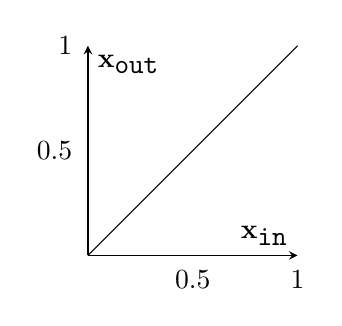
\begin{tikzpicture}
    \begin{axis}[
            width=0.35\textwidth,
            height=0.35\textwidth,
            xlabel={$\xin$},
            ylabel={$\xout$},
            axis lines=center,
            xtick distance=0.5,
            ytick distance=0.5,
            tick style={draw=none},
            xmin=0,xmax=1,
            ymin=0,ymax=1
    ]
    
    \addplot +[mark=none,smooth,black] {x};
    
    \end{axis}
\end{tikzpicture}
\end{figure}

In this chapter, we will instead consider a different way of plotting the mapping, where we simply rotate the y-axis to be horizontal rather than vertical:

\begin{figure}[h]
\centering
\begin{minipage}[t][4.5cm][c]{0.35\textwidth}
\begin{tikzpicture}
    \begin{axis}[
            width=1.0\textwidth,
            height=1.0\textwidth,
            xlabel={$\xin$},
            ylabel={$\xout$},
            axis lines=center,
            tick style={draw=none},
            xtick distance=0.5,
            ytick distance=0.5,
            xmin=0,xmax=1,
            ymin=0,ymax=1,
    ]
    
    \addplot +[mark=none,smooth,black] {x};
    
    \addplot[scatter src=explicit symbolic, only marks, mark=triangle*, mark options={rotate=90}] coordinates {
        (0.03,0.1)
        (0.03,0.2)
        (0.03,0.3)
        (0.03,0.4)
        (0.03,0.5)
        (0.03,0.6)
        (0.03,0.7)
        (0.03,0.8)
    };
    
    \addplot[scatter src=explicit symbolic, only marks, mark=*] coordinates {
        (0.1,0)
        (0.2,0)
        (0.3,0)
        (0.4,0)
        (0.5,0)
        (0.6,0)
        (0.7,0)
        (0.8,0)
    };
    
    \addplot[mark=none,dashed] coordinates {
    	(0.1,0)
    	(0.1,0.1)
    };
    \addplot[mark=none,dashed] coordinates {
    	(0.2,0)
    	(0.2,0.2)
    };
    \addplot[mark=none,dashed] coordinates {
    	(0.3,0)
    	(0.3,0.3)
    };
    \addplot[mark=none,dashed] coordinates {
    	(0.4,0)
    	(0.4,0.4)
    };
    \addplot[mark=none,dashed] coordinates {
    	(0.5,0)
    	(0.5,0.5)
    };
    \addplot[mark=none,dashed] coordinates {
    	(0.6,0)
    	(0.6,0.6)
    };
    \addplot[mark=none,dashed] coordinates {
    	(0.7,0)
    	(0.7,0.7)
    };
    \addplot[mark=none,dashed] coordinates {
    	(0.8,0)
    	(0.8,0.8)
    };
    
    \addplot[mark=none,dashed] coordinates {
    	(0,0.1)
    	(0.1,0.1)
    };
    \addplot[mark=none,dashed] coordinates {
    	(0,0.2)
    	(0.2,0.2)
    };
    \addplot[mark=none,dashed] coordinates {
    	(0,0.3)
    	(0.3,0.3)
    };
    \addplot[mark=none,dashed] coordinates {
    	(0,0.4)
    	(0.4,0.4)
    };
    \addplot[mark=none,dashed] coordinates {
    	(0,0.5)
    	(0.5,0.5)
    };
    \addplot[mark=none,dashed] coordinates {
    	(0,0.6)
    	(0.6,0.6)
    };
    \addplot[mark=none,dashed] coordinates {
    	(0,0.7)
    	(0.7,0.7)
    };
    \addplot[mark=none,dashed] coordinates {
    	(0,0.8)
    	(0.8,0.8)
    };
    
\end{axis}
\end{tikzpicture}
\end{minipage}
\begin{minipage}[t][4.5cm][c]{0.1\textwidth}
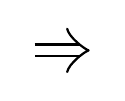
\begin{tikzpicture}
    \draw [line width=1pt, double distance=3pt, -{Classical TikZ Rightarrow[length=3mm]}] (0,0) -- (0.7,0);
\end{tikzpicture}
\end{minipage}
\begin{minipage}[t][4.5cm][c]{0.35\textwidth}
\begin{tikzpicture}
    \begin{axis}[
            rep2rep axis style,
            xlabel={$\xin$},
    ]
    \end{axis}
    
    \begin{axis}[
            rep2rep axis style,
            xlabel={$\xout$},
            axis lines=top,
    ]
    
    \addplot[mark=none,dashed] coordinates {
    	(0.1,0)
    	(0.1,1)
    };
    \addplot[mark=none,dashed] coordinates {
    	(0.2,0)
    	(0.2,1)
    };
    \addplot[mark=none,dashed] coordinates {
    	(0.3,0)
    	(0.3,1)
    };
    \addplot[mark=none,dashed] coordinates {
    	(0.4,0)
    	(0.4,1)
    };
    \addplot[mark=none,dashed] coordinates {
    	(0.5,0)
    	(0.5,1)
    };
    \addplot[mark=none,dashed] coordinates {
    	(0.6,0)
    	(0.6,1)
    };
    \addplot[mark=none,dashed] coordinates {
    	(0.7,0)
    	(0.7,1)
    };
    \addplot[mark=none,dashed] coordinates {
    	(0.8,0)
    	(0.8,1)
    };
    \addplot[mark=none,dashed] coordinates {
    	(0.9,0)
    	(0.9,1)
    };
    
    \addplot[scatter src=explicit symbolic, only marks, mark=*] coordinates {
        (0.1,0)
        (0.2,0)
        (0.3,0)
        (0.4,0)
        (0.5,0)
        (0.6,0)
        (0.7,0)
        (0.8,0)
        (0.9,0)
    };
    
    \addplot[scatter src=explicit symbolic, only marks, mark=triangle*] coordinates {
        (0.1,0.97)
        (0.2,0.97)
        (0.3,0.97)
        (0.4,0.97)
        (0.5,0.97)
        (0.6,0.97)
        (0.7,0.97)
        (0.8,0.97)
        (0.9,0.97)
    };
    
\end{axis}
\end{tikzpicture}
\end{minipage}
\end{figure}

The depiction to the right makes it obvious that the plot $\xout = \xin$ is the identity mapping: datapoints get mapped to unchanged positions. Here are a few more mappings plotted in this way:

\begin{figure}[h]
\centering
\begin{minipage}[t][5.5cm][c]{0.45\textwidth}
\begin{flushleft}
\begin{tikzpicture}
    \begin{axis}[
            rep2rep axis style,
            width=0.78\textwidth,
            height=0.78\textwidth,
            title={$\xout = 2\xin$},
            title style={at={(0.1,0.5)},anchor=north east,draw=black,fill=white},
            xlabel={$\xin$},
            xmin=-1.2,xmax=1.2,
    ]
    \end{axis}
    
    \begin{axis}[
            rep2rep axis style,
            width=0.78\textwidth,
            height=0.78\textwidth,
            xlabel={$\xout$},
            axis lines=top,
            xmin=-1.2,xmax=1.2,
    ]
    
    \addplot[mark=none,dashed] coordinates {
    	(-0.5,0)
    	(-1.0,1)
    };
    \addplot[mark=none,dashed] coordinates {
    	(-0.25,0)
    	(-0.5,1)
    };
    \addplot[mark=none,dashed] coordinates {
    	(0,0)
    	(0,1)
    };
    \addplot[mark=none,dashed] coordinates {
    	(0.25,0)
    	(0.5,1)
    };
    \addplot[mark=none,dashed] coordinates {
    	(0.5,0)
    	(1,1)
    };
    
    \addplot[scatter src=explicit symbolic, only marks, mark=*] coordinates {
        (-0.5,0)
        (-0.25,0)
        (0,0)
        (0.25,0)
        (0.5,0)
    };
    
    \addplot[scatter src=explicit symbolic, only marks, mark=triangle*] coordinates {
        (-1,0.97)
        (-0.5,0.97)
        (0,0.97)
        (0.5,0.97)
        (1,0.97)
    };
    
\end{axis}
\end{tikzpicture}
\end{flushleft}
\end{minipage}
\begin{minipage}[t][5.5cm][c]{0.45\textwidth}
\begin{flushright}
\begin{tikzpicture}
    \begin{axis}[
            rep2rep axis style,
            width=0.78\textwidth,
            height=0.78\textwidth,
            title={$\xout = \frac{\xin + 1}{2}$},
            title style={at={(0.1,0.5)},anchor=north east,draw=black,fill=white},
            xlabel={$\xin$},
            xmin=-1.2,xmax=1.2,
    ]
    \end{axis}
    
    \begin{axis}[
            rep2rep axis style,
            width=0.78\textwidth,
            height=0.78\textwidth,
            xlabel={$\xout$},
            axis lines=top,
            xmin=-1.2,xmax=1.2,
    ]
    
    \addplot[mark=none,dashed] coordinates {
    	(-1.0,0)
    	(0,1)
    };
    \addplot[mark=none,dashed] coordinates {
    	(-0.5,0)
    	(0.25,1)
    };
    \addplot[mark=none,dashed] coordinates {
    	(0,0)
    	(0.5,1)
    };
    \addplot[mark=none,dashed] coordinates {
    	(0.5,0)
    	(0.75,1)
    };
    \addplot[mark=none,dashed] coordinates {
    	(1,0)
    	(1,1)
    };
    
    \addplot[scatter src=explicit symbolic, only marks, mark=*] coordinates {
        (-1,0)
        (-0.5,0)
        (0,0)
        (0.5,0)
        (1,0)
    };
    
    \addplot[scatter src=explicit symbolic, only marks, mark=triangle*] coordinates {
        (0,0.97)
        (0.25,0.97)
        (0.5,0.97)
        (0.75,0.97)
        (1,0.97)
    };
    
\end{axis}
\end{tikzpicture}
\end{flushright}
\end{minipage}
\begin{minipage}[t][5.5cm][c]{0.45\textwidth}
\begin{flushleft}
\begin{tikzpicture}
    \begin{axis}[
            rep2rep axis style,
            width=0.78\textwidth,
            height=0.78\textwidth,
            title={$\xout = \texttt{relu}(\xin)$},
            title style={at={(0.1,0.5)},anchor=north east,draw=black,fill=white},
            xlabel={$\xin$},
            xmin=-1.2,xmax=1.2,
    ]
    \end{axis}
    
    \begin{axis}[
            rep2rep axis style,
            width=0.78\textwidth,
            height=0.78\textwidth,
            xlabel={$\xout$},
            axis lines=top,
            xmin=-1.2,xmax=1.2,
    ]
    
    \addplot[mark=none,dashed] coordinates {
    	(-1,0)
    	(0,1)
    };
    \addplot[mark=none,dashed] coordinates {
    	(-0.5,0)
    	(0,1)
    };
    \addplot[mark=none,dashed] coordinates {
    	(0,0)
    	(0,1)
    };
    \addplot[mark=none,dashed] coordinates {
    	(0.5,0)
    	(0.5,1)
    };
    \addplot[mark=none,dashed] coordinates {
    	(1,0)
    	(1,1)
    };
    
    \addplot[scatter src=explicit symbolic, only marks, mark=*] coordinates {
        (-1,0)
        (-0.5,0)
        (0,0)
        (0.5,0)
        (1,0)
    };
    
    \addplot[scatter src=explicit symbolic, only marks, mark=triangle*] coordinates {
        (0,0.97)
        (0.5,0.97)
        (0,0.97)
        (0.5.5,0.97)
        (1, 0.97)
    };
    
\end{axis}
\end{tikzpicture}
\end{flushleft}
\end{minipage}
\begin{minipage}[t][5.5cm][c]{0.45\textwidth}
\begin{flushright}
\begin{tikzpicture}
    \begin{axis}[
            rep2rep axis style,
            width=0.78\textwidth,
            height=0.78\textwidth,
            title={$\xout = \texttt{sigmoid}(\xin)$},
            title style={at={(0.1,0.5)},anchor=north east,draw=black,fill=white},
            xlabel={$\xin$},
            xmin=-5.2,xmax=5.2,
            xtick distance=2.5,
    ]
    \end{axis}
    
    \begin{axis}[
            rep2rep axis style,
            width=0.78\textwidth,
            height=0.78\textwidth,
            xlabel={$\xout$},
            axis lines=top,
            xmin=-1.2,xmax=1.2,
    ]
    
    \addplot[mark=none,dashed] coordinates {
    	(-1.0,0)
    	(0.007,1)
    };
    \addplot[mark=none,dashed] coordinates {
    	(-0.5,0)
    	(0.076,1)
    };
    \addplot[mark=none,dashed] coordinates {
    	(0,0)
    	(0.5,1)
    };
    \addplot[mark=none,dashed] coordinates {
    	(0.5,0)
    	(0.924,1)
    };
    \addplot[mark=none,dashed] coordinates {
    	(1,0)
    	(0.993,1)
    };
    
    \addplot[scatter src=explicit symbolic, only marks, mark=*] coordinates {
        (-1,0)
        (-0.5,0)
        (0,0)
        (0.5,0)
        (1,0)
    };
    
    \addplot[scatter src=explicit symbolic, only marks, mark=triangle*] coordinates {
        (0.007,0.97)
        (0.076,0.97)
        (0.5,0.97)
        (0.924,0.97)
        (0.993,0.97)
    };
    
\end{axis}
\end{tikzpicture}
\end{flushright}
\end{minipage}
\end{figure}

Each of the above are layers that could be found in a deep net. Linear layers, like those in the top row above, stretch and squash the data distribution. The \texttt{relu} nonlinearity maps all negative data to 0, and applies an identity map to all non-negative data. The \texttt{sigmoid} function pulls negative data to 0 and positive data to 1.

In this way, an incoming data distribution can be reshaped layer by layer into a desired configuration. The goal a binary classifier, for example, is to move the datapoints around until all the class 0 points end up moved to 0 on the output layer and all the class 1 end up moved to 1.

A deep net stacks these operations, like so:
\begin{figure}[h]
\centering
\begin{tikzpicture}
    \begin{axis}[
            rep2rep axis style,
            width=0.35\textwidth,
            height=0.4\textwidth,
            title={$\mathbf{x}^{(1)} = 2*\mathbf{x}^{(0)}$},
            title style={at={(0.1,0.25)},anchor=north east,draw=black,fill=white},
            xlabel={$\mathbf{x}^{(0)}$},
            xmin=-1.2,xmax=1.2,
    ]
    \end{axis}
    
    % \begin{axis}[
    %         rep2rep axis style,
    %         width=0.35\textwidth,
    %         height=0.25\textwidth,
    %         title={$\mathbf{x}^{(2)} = \texttt{relu}(\mathbf{x}^{(1)})$},
    %         title style={at={(0.1,1.5)},anchor=north east,draw=black,fill=white},
    %         xlabel={$\mathbf{x}^{(1)}$},
    %         axis lines=top,
    %         xmin=-1.2,xmax=1.2,
    % ]
    % \end{axis}
    
    \begin{axis}[
            rep2rep axis style,
            width=0.35\textwidth,
            height=0.4\textwidth,
            title={$\mathbf{x}^{(2)} = \texttt{relu}(\mathbf{x}^{(1)})$},
             title style={at={(0.1,0.75)},anchor=north east,draw=black,fill=white},
            xlabel={$\mathbf{x}^{(2)}$},
            axis lines=top,
            xmin=-1.2,xmax=1.2,
            ymin=0,ymax=2
    ]
    
    \addplot[mark=none] coordinates {
    	(-1.2,1)
    	(1.2,1)
    };
    
    \addplot[mark=none,dashed] coordinates {
    	(-0.5,0)
    	(-1.0,1)
    };
    \addplot[mark=none,dashed] coordinates {
    	(-0.25,0)
    	(-0.5,1)
    };
    \addplot[mark=none,dashed] coordinates {
    	(0,0)
    	(0,1)
    };
    \addplot[mark=none,dashed] coordinates {
    	(0.25,0)
    	(0.5,1)
    };
    \addplot[mark=none,dashed] coordinates {
    	(0.5,0)
    	(1,1)
    };
    
    \addplot[scatter src=explicit symbolic, only marks, mark=*] coordinates {
        (-0.5,0)
        (-0.25,0)
        (0,0)
        (0.25,0)
        (0.5,0)
    };
    
    \addplot[scatter src=explicit symbolic, only marks, mark=triangle*] coordinates {
        (-1,0.97)
        (-0.5,0.97)
        (0,0.97)
        (0.5,0.97)
        (1,0.97)
    };
    
    \addplot[mark=none,dashed] coordinates {
    	(-1,1)
    	(0,2)
    };
    \addplot[mark=none,dashed] coordinates {
    	(-0.5,1)
    	(0,2)
    };
    \addplot[mark=none,dashed] coordinates {
    	(0,1)
    	(0,2)
    };
    \addplot[mark=none,dashed] coordinates {
    	(0.5,1)
    	(0.5,2)
    };
    \addplot[mark=none,dashed] coordinates {
    	(1,1)
    	(1,2)
    };
    
    \addplot[scatter src=explicit symbolic, only marks, mark=triangle*] coordinates {
        (0,1.97)
        (0,1.97)
        (0,1.97)
        (0.5,1.97)
        (1,1.97)
    };
    
\end{axis}

\end{tikzpicture}
\end{figure}


\section{2D representations}

A nice property of the above way of plotting is that it also extends to visualizing 2D-to-2D mappings (something that conventional x-axis/y-axis plotting is not well equipped to do). Real deep nets perform ND-to-ND mappings, but already 2D-to-2D visualizations can give a lot of insight into the general case.

Here is a linear layer $f: \mathbb{R}^2 \rightarrow \mathbb{R}^2$:

\begin{figure}[h]
    \centering
    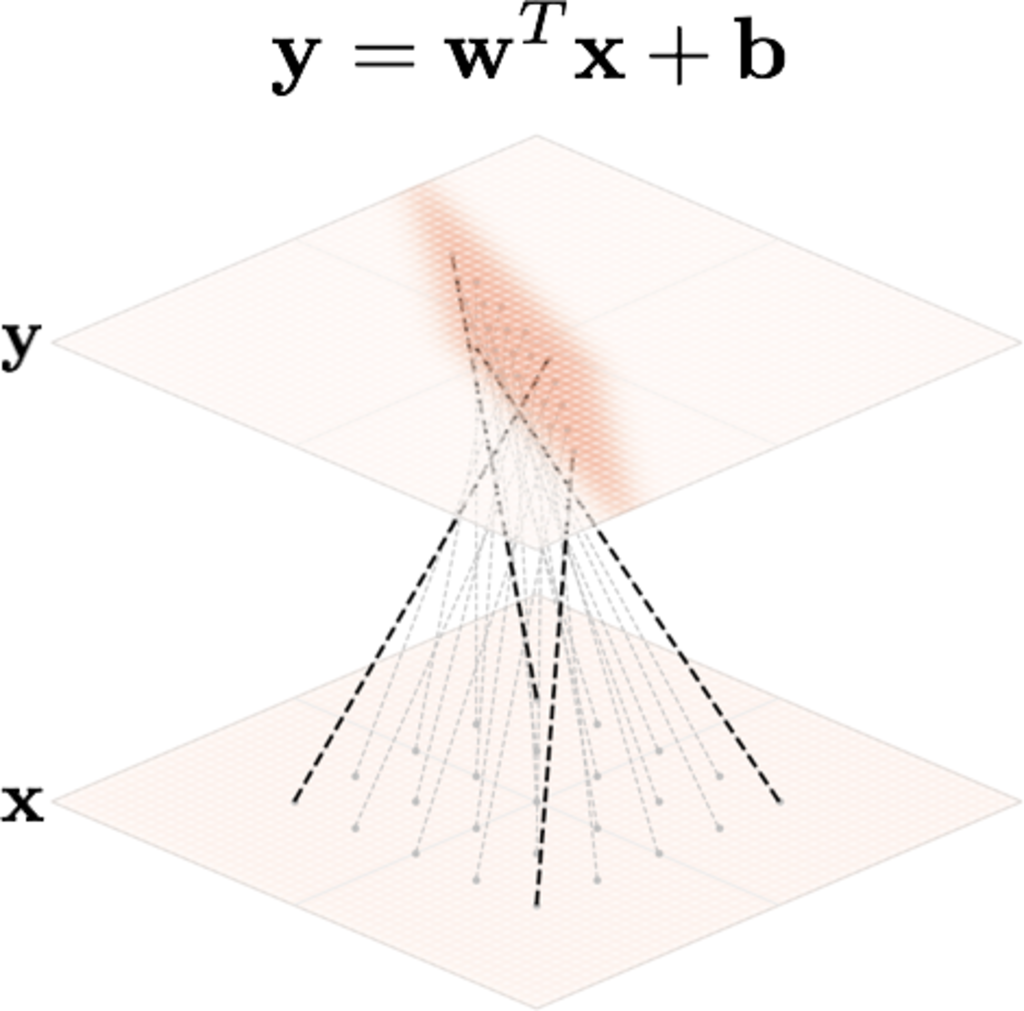
\includegraphics[width=0.36\linewidth]{./figures/neural_nets_as_data_transformations/2D_linear_layer.png}
    \label{fig:neural_nets_as_data_transformations:2D_linear_layer}
\end{figure}

\section{Deep nets as representation transformers}
The data can be thought of as itself a representation. The target output, e.g., class labels, is another representation. Then a classifier network, layer by layer, maps a representations that matches the raw data to a representation that matches the labels. The sequence of representations for an input datapoint $\xin^i$ is $\xin^i \rightarrow \mathbf{h}^{(1)i} \rightarrow \mathbf{h}^{(2)i} \rightarrow \cdots \rightarrow \xout^i$.

One way to characterize this sequence of representations is by looking at how each subsequent layer represents an entire \emph{dataset}. 


\section{Deep nets as distribution transformers}
The plots from the previous section show how a uniform grid of datapoints get mapped from layer to layer in a deep net. We can also use this plotting style to show how a different distribution of incoming datapoints gets transformed. This is the setting in which deep nets actually operate, and sometimes the real action of the network looks very different when viewed this way. We can think of a deep net as transforming an input data distribution, $\pdata$, into an output data distribution, $\pout$. In fact, each layer of activations in a network is a different representation of the data, and we can consider the distribution of activations on some layer $\ell$ to be $p_{\ell}$. Then, layer by layer, a deep net transforms $\pdata$ into $p_{\texttt{1}}$ into $p_{\texttt{2}}$, and so on until finally transforming the data to the distribution $\pout$.


%Each layer of a deep net performs a mapping that moves the datapoints around.







\section{Representations beyond 2D}
For example, if the representation $\mathbf{h}^{(1)i}$ were a two-dimensional vector, then we could visualize this representation for all datapoints $i$ in a dataset as a 2D scatter plot. If the next layer $\mathbf{h}^{(2)i}$ were also two-dimensional, then it would be a different scatter plot, with each datapoint shifted to a new position. Typically, each hidden layer is a high-dimensional vector, so it's non-trivial to visualize datapoints in this space. However, we may apply tools from {\bf dimensionality reduction} to show a 2D projection of the data, such that the distance between two datapoints in the 2D projection is roughly proportional to their actual distance in the high-dimensional space. The below plot, reproduced from \cite{decaf}, uses a dimensionality reduction technique called t-SNE~\cite{tsne} to visualize how different layers of a deep net represent a dataset of images of different semantic classes, where each color represents a different semantic class:

\begin{figure}[h]
    \centering
    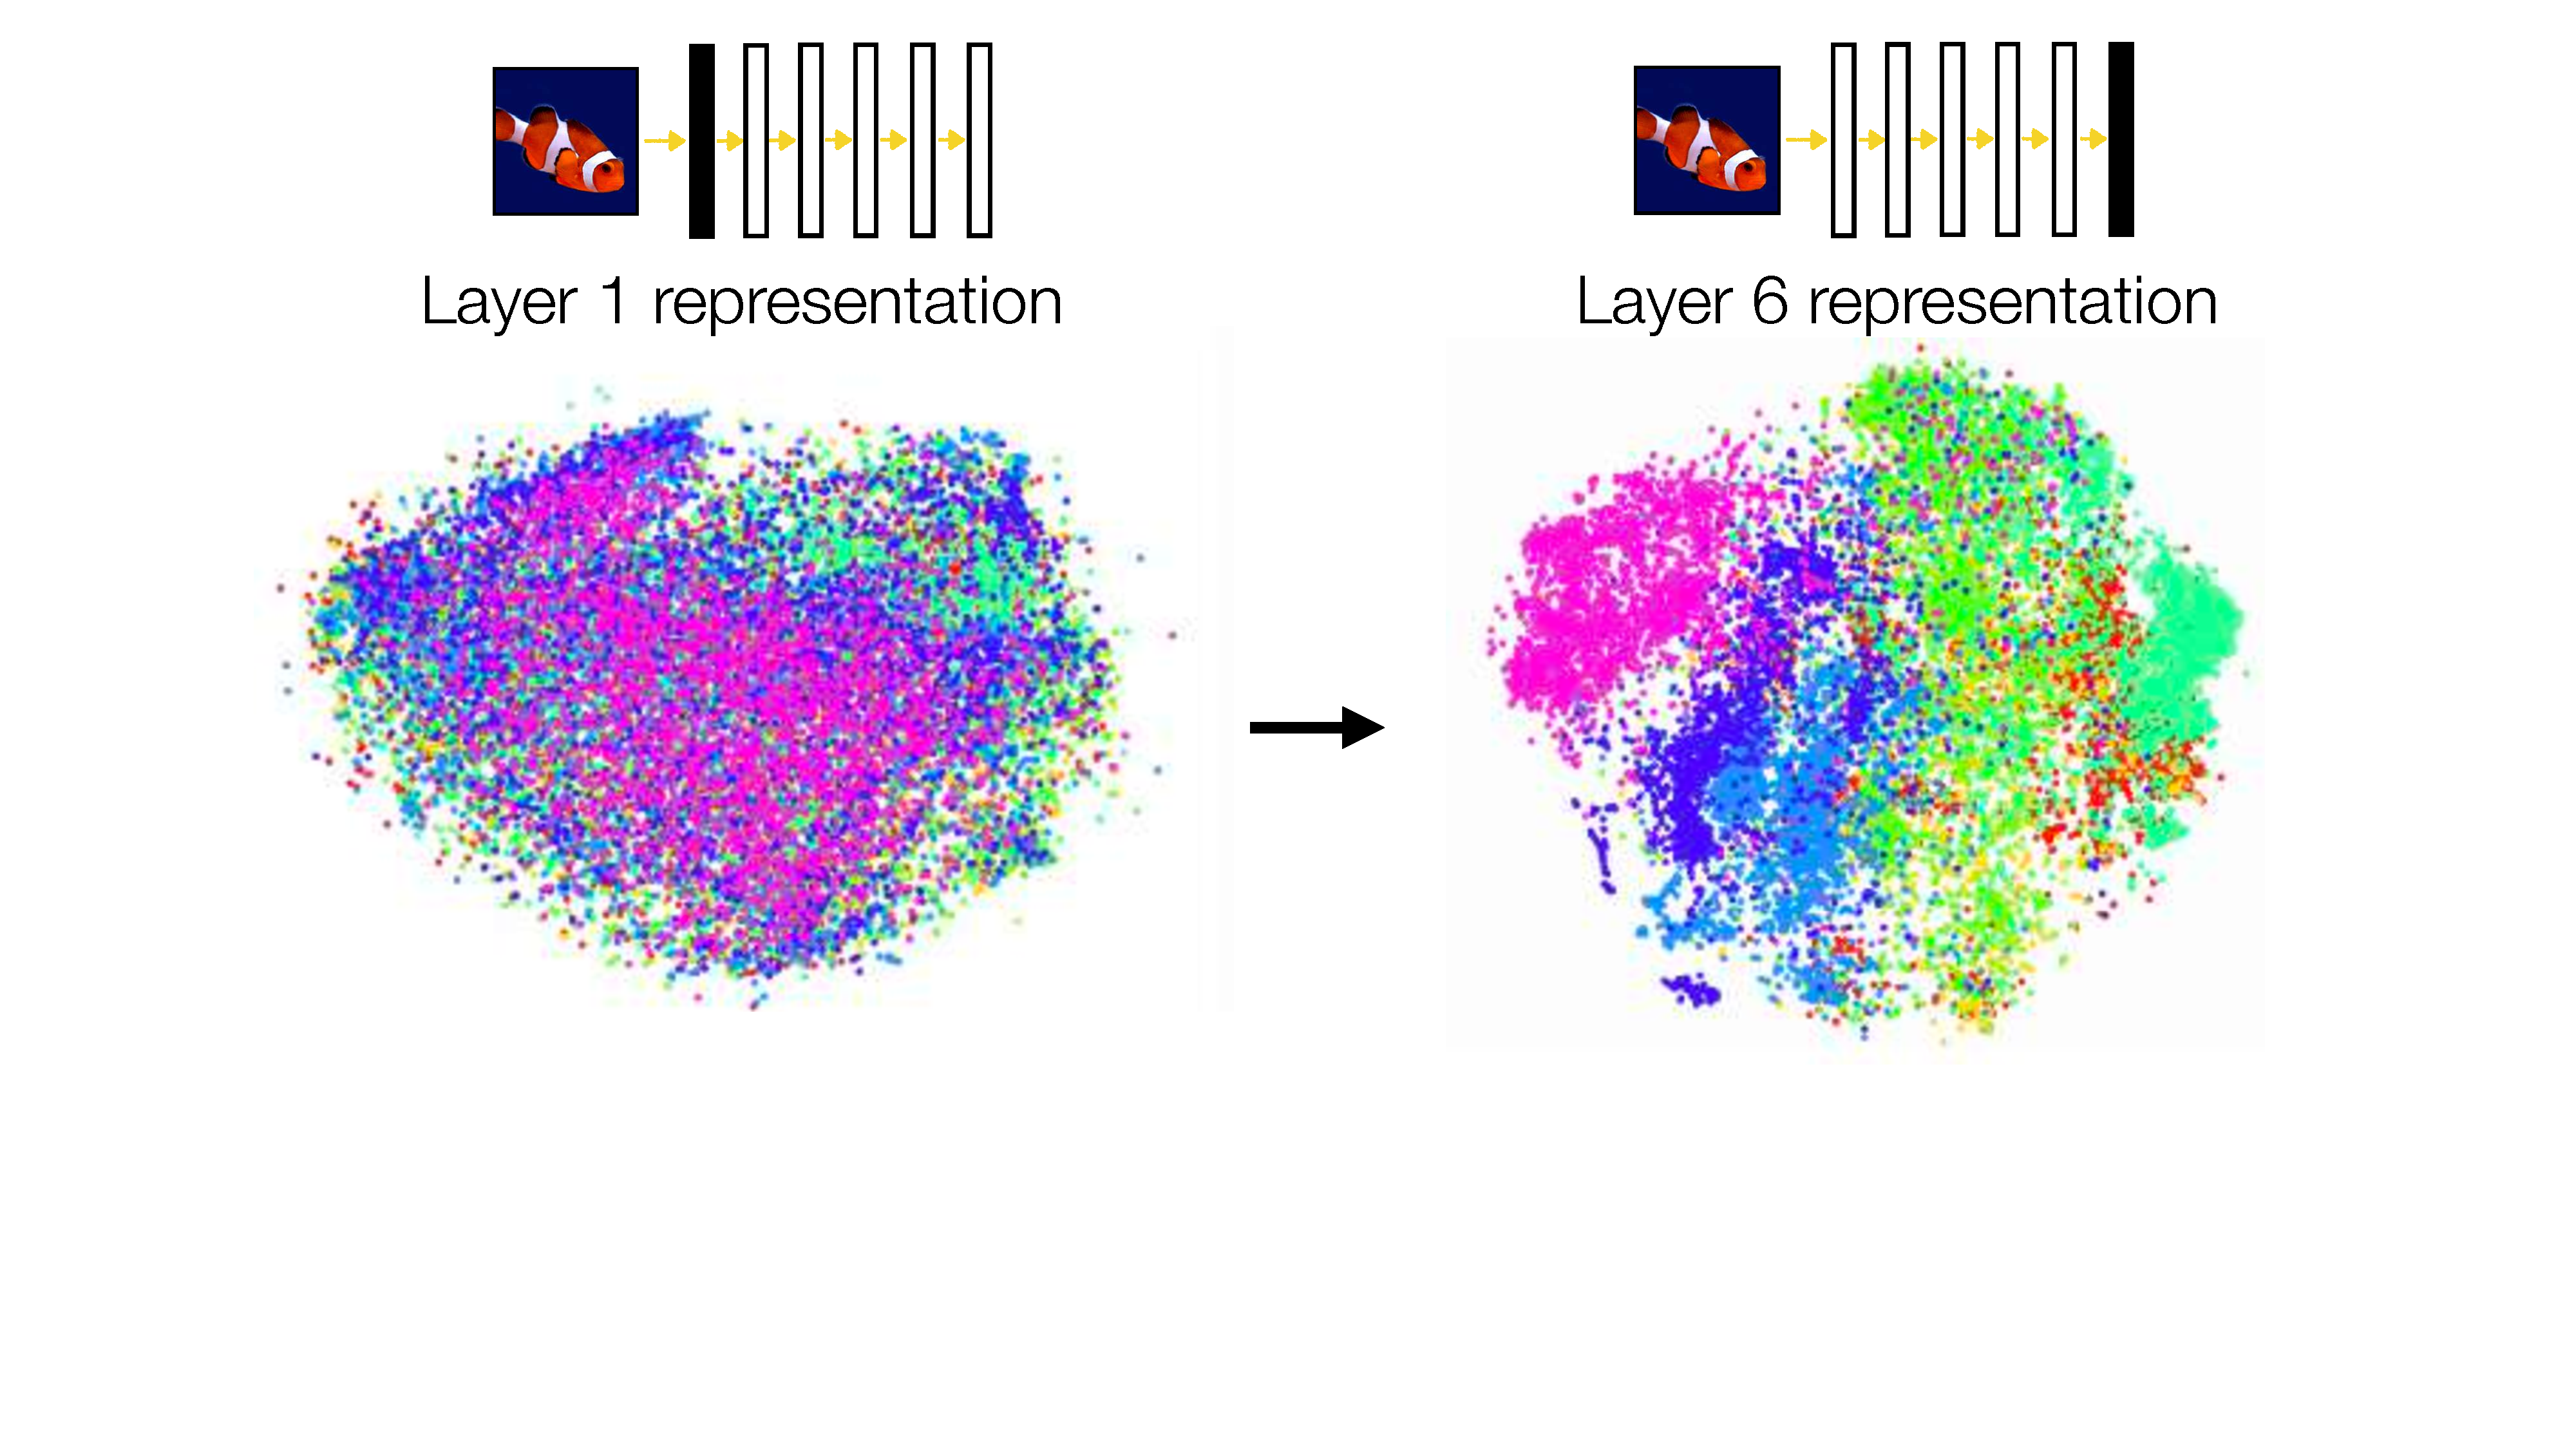
\includegraphics[width=0.6\linewidth]{./figures/neural_nets/decaf_tsne.pdf}
    \label{fig:decaf_tsne}
\end{figure}

Notice that on the first layer, semantic classes are not well separated but by layer 6 the representation has {\bf disentangled} the semantic classes so that each class occupies a different part of representational space. This is expected because layer 6 is near the output of the network, and the output is being trained to be a one-hot representation of semantics -- i.e. a completely disentangled representation.
